% vim: spell spelllang=en:
%! TEX root = **/00-main.tex

% PCA analysis for numerical variables:

\section{PCA analysis for numerical variables}%
\label{sec:pca_analysis_for_numerical_variables}

% Scree plot. Specify how many principal components are selected
\subsection{Scree plot}%
\label{sub:scree_plot}


\begin{figure}[H]
    \centering
    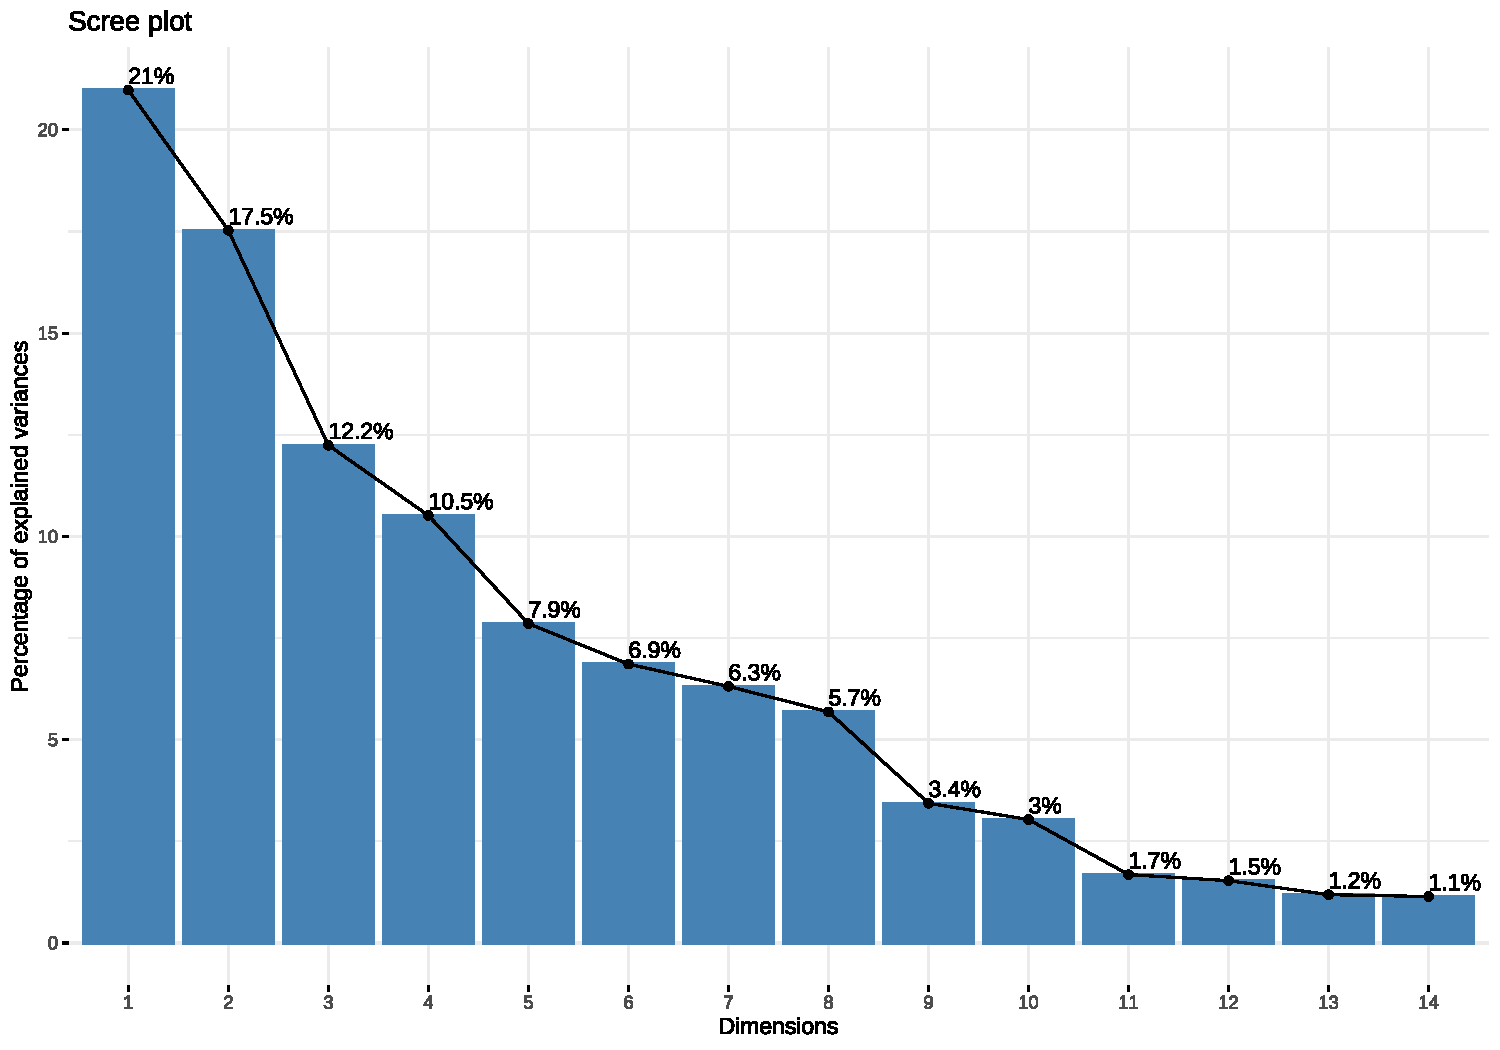
\includegraphics[width=0.7\linewidth]{pca_fact-screeplot} % PCA-inertia_cum
    \caption{PCA inertia}%
    \label{fig:pca_inertia}
\end{figure}

\begin{figure}[H]
    \centering
    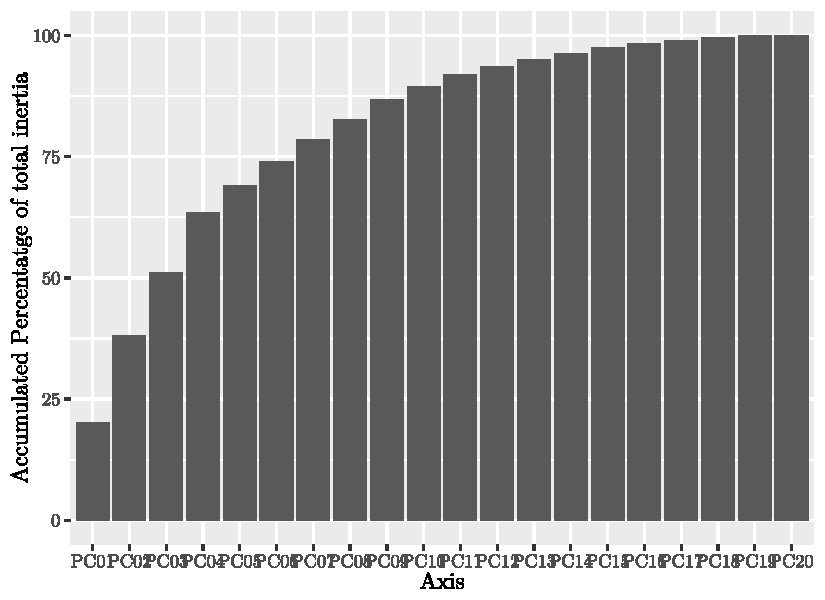
\includegraphics[width=0.7\linewidth]{PCA-inertia_cum}
    \caption{PCA accumulated inertia}%
    \label{fig:pca_inertia_cum}
\end{figure}

\vspace{-1em}
We used the inertia plots to decide the number of factorial axis to analyse. In
\cref{fig:pca_inertia} we can conclude the 4 first axis represent a much
larger amount of variance compared to the others. When looking at
\cref{fig:pca_inertia_cum} we can see that the first 4 axis already contain 61\%
of the variance. If we analyse further with the elbow method we can clearly see
that the slop starts to decrease at around the 4\ts{th} axis. Therefore we decided to
only further analyse the first 4 factorial axis.

% 20.24968405 17.88042469 13.04514781 12.39547495
% 20.24968  38.13011  51.17526  63.57073     %  69.09301  74.04671  78.51992  82.73880

\begin{table}[H]
    \centering
    \caption{Eigenvalues \& variance percentage of first 5 Dimensions}%
    \label{tab:eig}
    
\begin{tabular}[t]{lrrr}
\toprule
  & Eigenvalue & Var. \% & Cum. Var. \%\\
\midrule
comp 1 & 4.0499368 & 20.249684 & 20.24968\\
comp 2 & 3.5760849 & 17.880425 & 38.13011\\
comp 3 & 2.6090296 & 13.045148 & 51.17526\\
comp 4 & 2.4790950 & 12.395475 & 63.57073\\
comp 5 & 1.1044548 & 5.522274 & 69.09301\\
\addlinespace
comp 6 & 0.9907408 & 4.953704 & 74.04671\\
comp 7 & 0.8946421 & 4.473211 & 78.51992\\
comp 8 & 0.8437760 & 4.218880 & 82.73880\\
comp 9 & 0.8078400 & 4.039200 & 86.77800\\
comp 10 & 0.5511517 & 2.755759 & 89.53376\\
\bottomrule
\end{tabular}
\end{table}

\begin{table}[H]
    \centering
    \caption{Variable contribution to each axis}%
    \label{tab:}
    
\begin{tabular}[t]{lrrrr}
\toprule
  & Dim.1 & Dim.2 & Dim.3 & Dim.4\\
\midrule
host\_listings\_count & 1.1978839 & 0.2309859 & 1.2348477 & 1.9194330\\
accommodates & 1.7298781 & 4.9204820 & 15.4579382 & 8.8411427\\
bedrooms & 1.5035858 & 3.8248072 & 14.2067930 & 10.2701716\\
beds & 1.5539744 & 4.1550603 & 14.5044651 & 9.4446670\\
price & 0.3358423 & 0.5034663 & 1.7979068 & 2.5310976\\
\addlinespace
minimum\_nights\_avg\_ntm & 0.3285224 & 0.1053913 & 0.8458848 & 1.3083557\\
maximum\_nights\_avg\_ntm & 0.0326754 & 0.1551460 & 0.0180542 & 0.1915016\\
availability\_30 & 4.7100532 & 13.9585375 & 7.7416460 & 0.0782981\\
availability\_60 & 5.0921343 & 15.0338778 & 8.3809077 & 0.0804272\\
availability\_90 & 5.0164904 & 15.0703072 & 8.1727252 & 0.0732742\\
\addlinespace
availability\_365 & 3.9814077 & 9.6538067 & 2.9478169 & 0.0828489\\
number\_of\_reviews & 1.3671328 & 5.0656577 & 6.0696363 & 12.6128426\\
number\_of\_reviews\_ltm & 1.4742472 & 5.9390691 & 6.6049015 & 15.9807855\\
number\_of\_reviews\_l30d & 0.3293267 & 1.6735082 & 1.7305596 & 5.7081947\\
review\_scores\_rating & 16.2922433 & 2.7642390 & 1.0363407 & 3.3113763\\
\addlinespace
review\_scores\_accuracy & 15.2310328 & 2.7062625 & 0.7857840 & 2.4644208\\
review\_scores\_cleanliness & 12.6689566 & 3.1473241 & 0.5491346 & 2.7145276\\
review\_scores\_location & 9.5058782 & 2.5671720 & 0.4498178 & 1.7099762\\
review\_scores\_value & 15.7847912 & 2.5825171 & 1.1601061 & 2.4687109\\
reviews\_per\_month & 1.8639432 & 5.9423821 & 6.3047340 & 18.2079477\\
\bottomrule
\end{tabular}
\end{table}

% Factorial map visualisation:
\subsection{Factorial map visualisation}%
\label{sub:factorial_map_visualisation}

\newcommand{\centroidmap}[2]{
    \begin{figure}[H]
        \centering
        \includegraphics[width=0.87\linewidth]{pca_fact-plane_#1_#2-cent}
        \caption{PCA plane #1 vs #2 (categorical variables centroids)}%
        \label{fig:plane_#1-#2-cent}
    \end{figure}
}

% #2 -> caption #3 -> file, #1 -> page
\newcommand{\factorialmap}[2]{
    \begin{landscape}
    \begin{figure}[H]
        \centering
        \includegraphics[width=0.87\linewidth]{pca_fact-plane_#1_#2-bi}
        \caption{PCA plane #1 vs #2}%
        \label{fig:plane_#1-#2}
    \end{figure}
    \end{landscape}
}

\newcommand{\factvar}[2]{
    \begin{figure}[H]
        \centering
        \includegraphics[width=0.67\textwidth]{pca_fact-plane_#1_#2-var}
        \caption{PCA plane #1 vs #2 (numerical)}%
        \label{fig:plane_#1-#2-var}
    \end{figure}
}

\newcommand{\factorialmapCV}[2]{
    \contrib{#1}{#2}
    \factvar{#1}{#2}
}

\newcommand{\contrib}[2]{
    \begin{figure}[H]
        \centering
        \includegraphics[width=0.85\linewidth]{pca_fact-plane_#1_#2-contrib}
        \caption{PCA variable contributions of plane #1 vs #2}%
        \label{fig:contrib_plane_#1-#2}
    \end{figure}
}

\newcommand{\categorica}[4]{
    \begin{figure}[H]
        \centering
        \includegraphics[width=0.85\linewidth]{pca_fact-#3-plane_#1_#2}
        \caption{PCA variable contributions of #4 in plane #1 vs #2}%
        \label{fig:cat-#3-plane-#1-#2}
    \end{figure}
}


\factorialmap{1}{2}
In \cref{fig:plane_1-2} we are showing the factorial maps that represent the most variance among all our factorial axis. When looking at the numerical variables represented we can see that all there are some variables that tend to be grouped. For example
there's a group about all review scores, another with beds, bedroom and accommodates and another with availabilities. When 
analysing \cref{fig:contrib_plane_1-2} we can see that accommodates, beds and the review scores are top contributors to
this plane. When analysing the contribution to each plane it's clear that review scores are affecting mostly axis 2, whereas accommodates and beds mostly affect axis 1.

\factorialmapCV{1}{2}


\factorialmap{1}{3}
In \cref{fig:plane_1-3} we can see that it seems to hold true that the accommodates and beds affects axis 1 the most. Price 
seems to have a similar arrow as those variables. This might be
because there is some correlation between those variables. 
(The more beds a house has, probably the more expensive it is).
The arrows of variables about number of reviews have a very small angle with factorial axis 3. Minimum\_nights\_avg\_ntm seem to
be affecting axis 3 as well but inversely.

\factorialmapCV{1}{3}

\factorialmap{1}{4}

In \cref{fig:plane_1-4} we can see that again it is true
the accommodates and beds variables affects axis 1 the most. We can begin to speculate that these might be factorial axis 1
latent variables. Looking at \cref{fig:contrib_plane_1-4} we 
can see that availabities first appear as top contributors and seem to be related with the forth factorial axis.

\factorialmapCV{1}{4}


\factorialmap{2}{3}
In \cref{fig:contrib_plane_2-3} the most contributing variables are the number of reviews and review scores. It is hard to extract some relation to any axis
from this plot because the variables seem to have contributions to both axis.

\factorialmapCV{2}{3}


\factorialmap{2}{4}

What we can extract when analysing \cref{fig:plane_2-4} is that the availability variables have 
a relatively high contribution and form a very small angle with the forth factorial axis. The same happens with review scores and the second axis.

\factorialmapCV{2}{4}


\factorialmap{3}{4}
We can't extract much more from \cref{fig:plane_3-4}. Everything
aforementioned seems to hold true in this specific plane.

\factorialmapCV{3}{4}

\begin{landscape}

\centroidmap{1}{2}

\categorica{1}{2}{room_type}{room type}
Looking at \cref{fig:cat-room_type-plane-1-2} that there are some 
differences between each room type category. As we explained in the PCA analysis of numerical variables, axis 1 is mostly affected by accommodates and bedrooms whereas the variables that contribute most to axis 2 are the review scores. If we analyse the
placement of centroids along the plane it seems to make sense as entire home/apt are supposed to have more bedrooms and capacities than a private room. If we analyse towards axis 2 we can see that entire homes and hotel rooms have better review scores than the 
other two. If we look at the variance of private rooms, represented by the ellipsis we 
can see that in general this category has less accommodates and bedrooms than the others.



\categorica{1}{2}{neighbourhood_group_cleansed}{Neighbourhood group}
Similarly to before, in \cref{fig:cat-neighbourhood_group_cleansed-plane-1-2} there seems to be some differences between Barcelona's neighborhoods in this plane. For example we can 
see that Nou Barris seem to have less accommodates and a worse review. On the other
hand l'Eixample has the most accommodates and the better reviews. When looking at
the ellipsis, which represent the 95\% interval of variance we can see that there are
some differences, specially when comparing the two examples given before. 

\categorica{2}{4}{host_is_superhost}{Host is superhost}
When looking at \cref{fig:cat-host_is_superhost-plane-2-4} we can
see that in general superhosts tend to have better reviews scores.

\categorica{2}{3}{host_since_year}{Host since year}
Looking at \cref{fig:cat-host_since_year-plane-2-3} we can see that the more recent hosts have less number of
reviews and lower review ratings.
The only exception is 2008 (which has no significance since it's only one individual).

\end{landscape}

\subsection{Conclusion}%
What we can conclude after analysing how the variables are distributed along each factorial axes is 
that our variables generally distribute in 4 groups: the ones about availability,   
the ones about review scores, the ones regarding number of reviews and finally beds and accommodation. That might indicate that there is some correlation between them.

After studying each factorial axis in depth we can conclude that each axes
latent variables associated to the first factorial map are the ones about accommodates and beds and the third factorial axis are mostly associated with 
the number of reviews. This is specially clear in \cref{fig:plane_1-3}. If we analyse the second factorial plane, it's latent variable isn't has clear cut.
However if we look at all planes with axis 2 and specially \cref{fig:plane_2-4}
we might speculate that it is mostly related to review scores. In this same figure we can see that the forth factorial plane is closely related to the availability.

When analysing the categorical variables we found out that most of them don't have many differences between their categories when projected in the factorial planes. Some interesting result were found in some of them. For example superhosts have better review scores or listings of entire houses and hotels have better accommodations and reviews than private rooms.

We conclude that the PCA visualization was an overall success because we were able to detect some grouped variables and relate some of them to our factorial axis. In fact we could more or less guess the latent variables related to
nearly all axes. This might be helpful in the future when analysing the clusters.


% (Be sure you use a single landscape pager for each single map in order to
% guarantee visibility of materials to the readers)

% For each factorial map provide:

% - Individuals projections

% - Common projection of numerical variables and modalities of qualitative
% - variables (take care to use correct color codes as explained along the course)

% - Interpretation of relationships among variables observed. When possible,
% - interpret the latent variable associated with the principal axis

% - Conclusions

% Note: All factorial maps must be placed in a single landscape page that makes
% it visible
